\documentclass[12pt, twoside]{article}

\usepackage{amsfonts}
%\usepackage[T1]{fontenc}
%\usepackage[ansinew]{inputenc}
\usepackage{amssymb}
\usepackage{amsthm}
\usepackage{amsmath}
% \usepackage{ mathrsfs }
\usepackage{dsfont}
\usepackage{natbib}
\setlength{\bibsep}{0pt plus 100ex}
\usepackage{url}
\usepackage{pdflscape}
\usepackage{pdfpages}
\usepackage{svg}
\usepackage[utf8]{inputenc}
\usepackage{graphicx}
\usepackage{bbold}
\usepackage{url}

\usepackage{rotating}
\usepackage{pdflscape}



\usepackage{enumitem}
%\usepackage[german,  onelanguage, linesnumbered]{algorithm2e}
\usepackage{placeins}
\usepackage{a4}
\usepackage[a4paper, ]{geometry}
\geometry{
 a4paper,
 right=30mm,
 left=30mm,
 top=30mm,
 }

% For tables
\usepackage{tabularx}
\usepackage{multirow}
\usepackage{pbox}

% \usepackage{color}

\widowpenalty = 5000
\clubpenalty = 5000


\newcommand{\Prob}{\mathbb{P}}
\newcommand{\V}{\mathbb{V}}
\newcommand{\Cov}{\text{Cov}}
\newcommand{\E}{\mathbb{E}}
\newcommand{\R}{\mathbb{R}}
\newcommand{\N}{\mathbb{N}}
\newcommand{\1}{\mathbb{1}}
\newcommand{\LL}{\mathcal{L}}
\newcommand{\F}{\mathcal{F}}
\newcommand{\iid}{\overset{\text{iid}}{\sim}}
\newcommand{\SUM}{\sum_{i=1}^n}
\newcommand{\PROD}{\prod_{i=1}^n}



\begin{document}

\begin{titlepage}

    \newcommand{\HRule}{\rule{\linewidth}{0.5mm}} % Defines a new command for the horizontal lines, change thickness here

    \center % Center everything on the page
 
    %----------------------------------------------------------------------------------------
    %	HEADING SECTIONS
    %----------------------------------------------------------------------------------------
    
\includegraphics[scale = 0.22]{campus-seal.jpg}\\[0.5cm]
    
     \textsc{\large University of California, Los Angeles}\\[0.2cm] % Minor heading such as course title
     \textsc{\large Department of Statistics}\\[0.5cm]
    %----------------------------------------------------------------------------------------
    %	TITLE SECTION
    %----------------------------------------------------------------------------------------

    \HRule \\[0.4cm]
    { \huge \bfseries Imputation of Missing Values in CART}\\[0.2cm] % Title of your document
    \HRule \\[0.4cm]
    \textsc{\large An Application of the EM Algorithm
    }\\[2.0 cm]
 
    %----------------------------------------------------------------------------------------
    %	AUTHOR SECTION
    %----------------------------------------------------------------------------------------
    
    \hspace{1cm}
    \begin{minipage}{0.4\textwidth}
    \begin{flushleft} \large
    \emph{Author:}\\
        Thomas \textsc{Maierhofer}\\
        SID 905078249 % Your name
    \end{flushleft}
    \end{minipage}
    ~
    \begin{minipage}{0.4\textwidth}
    \begin{flushright} \large
    \emph{Stats 201C:} \\
    Prof. Quing Zhou \\ % Supervisor's Name
    \text{}
    \end{flushright}
    \end{minipage}\\[1.5cm]
    
    \large{
    Final Project Report
    } \\[1.5cm]
    
    {\large Spring Quarter 2019,} \\
    {\large June 14, 2019}\\[2cm] % Date, change the \today to a set date if you want to be precise

    %----------------------------------------------------------------------------------------

    \vfill % Fill the rest of the page with whitespace

\end{titlepage}

%\newpage
%\hspace{5cm}
%\newpage

\pagenumbering{roman}
\tableofcontents 
\clearpage

\begin{abstract}
Classification and Regression Trees (CARTs) are one of the most widely used algorithms in machine learning. 
There are multiple ways of treating missing values in covariates, many of which work well in different scenarios. This report proposes a novel strategy for imputing missing values based on an EM algorithm. In the expectation step (E step), missing values are imputed based on the leaf node in which the corresponding observation falls given the current CART. In the maximization step (M step), the CART is fit on the current training data. These steps are repeated until convergence, i.e.\ the imputed values do not change anymore. 
Using a simulation study where missing values are introduced missing at random into a real data set, this EM algorithm is shown to achieve superior predictive performance in comparison with a number of standard approaches to handling missing values in CART.


\end{abstract}
\clearpage
\pagenumbering{arabic}

\section{Introduction}
This report introduces a novel approach to handling missing values in CARTs. It is structured as follows: Section~\ref{background} introduces CARTs and the EM algorithm, the two main concepts required for the proposed method for handling missing values in CARTs in Section~\ref{treatment_of_missing_values_in_cart}. Section~\ref{simulation_study} showcases the superior performanc in comparison with standard treatments of missing values in a real data set with artificially introduced missing values. The report ends with an outlook on potential future research in Section~\ref{futre_research}.

\section{Background}\label{background}
This section introduces the two cornerstones of this report: Classification and Regression Trees (CARTs) in Section~\ref{CART} and the EM algorithm in Section~\ref{EM_algorithm}. 

\subsection{Classification And Regression Trees}\label{CART}
CARTs were originally introduced by \cite{breiman1984} and have quickly gained popularity due to their competitive predictive power, ease of implementation, and compellingly simple concept.
CARTs create a model based on recursively splitting the covariate space into more homogeneous (w.r.t.\ the target variable) subspaces, a.k.a.\ nodes, using binary splits on individual covariates. The final nodes are called leaves and are used for prediction.
The basic algorithm for CART works as follows: \\

\fbox{ \centering{
\parbox{0.9\textwidth}{\textbf{Creating CART}
\begin{enumerate}
    \item Initialize empty tree with the root node containing all observations
    \item For each node not satisfying the stopping criterion: \label{step:CART_split}
    \begin{enumerate}[label*=\arabic*]
        \item Find the split that minimizes the node impurity in its resulting child nodes
        \item Add child nodes to the tree.
    \end{enumerate}
    \item While stopping criterion of the tree is not reached repeat Step~\ref{step:CART_split}
    \item Return tree with splits and nodes
\end{enumerate}
}}} 
\\

Note that all splits are binary splits on one of the covariates. Common stopping criteria for nodes are its minimal nodesize or minimal impurity. Nodes that are not split any further are called leaf nodes.
A common stopping criteria for the overall tree is its depth, i.e.\ maximal number of recursive splits. 
Common measures of node impurity are Gini Index for categorical target variables and MSE for numerical target variables.
% Most commonly, a CART is depicted in a tree structure, see Figure~TODO, but for two dimensional carts the splits can be shown in a planar colormap, see Figure~TODO.


\subsection{Expectation Maximization Algorithm}\label{EM_algorithm}
The EM algorithm is an iterative algorithm for obtaining the maximum likelihood estimator for parameters in a statistical model under the presence of unobserved variables. 
The basic concept of the EM algorithm has been used for a long time but was explicitly formalized by \cite{dempster1977maximum}.
The EM algorithm iterates until convergence between the expectation step (E step), where the parameters of the model are used to obtain the (expectation of) the unobserved variables, and the maximization step (M step), where the model parameters are chosen to maximize the likelihood given the estimated (originally unobserved, now observed) variables.

\section{Treatment of Missing Values in CART}\label{treatment_of_missing_values_in_cart}
This section introduces an EM algorithm for the treatment of missing values in CARTs in Section~\ref{EM_for_CART} after a brief review of commonly used methods in Section~\ref{traditional_methods}.

\subsection{Traditional Methods}\label{traditional_methods}
The most obvious way of treating missing values in a CART (and any other statistical model) is to simply delete observations with missing values. This is problematic if the data is not missing completely at random (MCAR) or if there are not enough complete pbservatiosn left to fit a reasonable model. 
Alternatively, missing values can be imputed using arithmetic means for scalar variables and modes for categorical variables. This ad-hoc method generally provides good results for MCAR data.
Both approaches are very problematic if the data is jsut missing at random (MAR) conditional on the observed data. This is a cmmon assumption, mainly because without it asymptotically true estimators cannot be obtained.

\subsection{EM Algorithm}\label{EM_for_CART}
The EM algorithm for the treatment of missing values in CARTs finds the maximum likelihood estimator for the model given its unobserved observations. It has the advantage, that asymptotically it will recover the true model parameters even if the missing values are MAR, i.e. they depend on the observed data.
In its E step, missing values are imputed based on the leaf node in which the observations falls given the current CART. Missing values in scalar covariates are imputed as the arithmetic mean of all observations within the leaf node, categorical covariates as the majority class (mode).
In its M step, the CART is fit on the current data. 
These steps are repeated until convergence, i.e.\ the imputed values do not change anymore. 
In pseudocode, this algorithm is:\\

\fbox{ \centering{
\parbox{0.9\textwidth}{\textbf{EM for Missing Values in CART}
\begin{enumerate}
    \item Initialize missing values as random draws from their (observed) marginal distribution
    \item Fit initial CART on completed data
    \item \textbf{E step}: Impute missing values as the covariates mean/mode in corresponding leaf node in current model \label{step:E_step}
    \item \textbf{M step}: Fit CART to current data \label{step:M_step} 
    \item Repeat Steps~\ref{step:E_step} and \ref{step:M_step} until convergence
\end{enumerate}
}}}
\\

\section{Simulation Study}\label{simulation_study}
The methodology proposed in Section~\ref{treatment_of_missing_values_in_cart} is compared using a simulations study.
The well known iris data set \citep{iris}, see Figure~\ref{fig:iris}, is used to have a realistic data generating process. A logistic regression model is used to introduce missing values (Section~\ref{missing_values}). The results of the performance comparison are summarized in Section~\ref{performance_comparison}.

\subsection{Introduction of Missing Values}\label{missing_values}
For the purpose of this simulation missing values are introduced into the iris data set at random (MAR). The probability of missing observation $X_{ij}$ for observation $i = 1, \ldots, n,$ and covariate $j = 1, \ldots, p,$, i.e. the propensity of $X_{ij}$, is sampled from a logistic regression model where the target variable is the indicator whether or not $X_{ij}$ is missing and the predictor variables are all other covariates $(X_{ik}), k \neq j$. The general model formula can be written as
\begin{eqnarray} \label{eq:missing_strategy}
P(X_{ij} \text{ missing}) &=& \text{logistic}(\beta_0 + \beta_1 X_{i1} + \ldots + \beta_{j - 1} X_{i(j - 1)} + \nonumber \\
&& \hspace{1.4cm}  \beta_{j + 1} X_{i(j + 1)} + \ldots + \beta_p X_{ip}),
\end{eqnarray}
where the model coefficients $\beta = (\beta_0, \beta_1, \ldots, \beta_{j - 1}, \beta_{j+1}, \ldots, \beta_p)$ are fixed and known simulation parameters.
Here, the parameter values $\beta = (0, 0.2, 0.4, -0.2, -0.2)$ corresponding to the intercept and the covariates "Sepal.Length", "Sepal.Width", "Petal.Length", and "Petal.Width", were chosen to achieve a high probability of missingness in the highly predictive covariates "Petal.Length" and "Petal.Width" and lower probabilities of missingness in "Sepal.Length", "Sepal.Width", in order to create a data set that was notably more difficult to train on than the fully observed data. The marginal shares of missing values sampled by this strategy are visualized in Figure~\ref{fig:marginal_missing}.

\begin{figure}[hp]
	\centering
	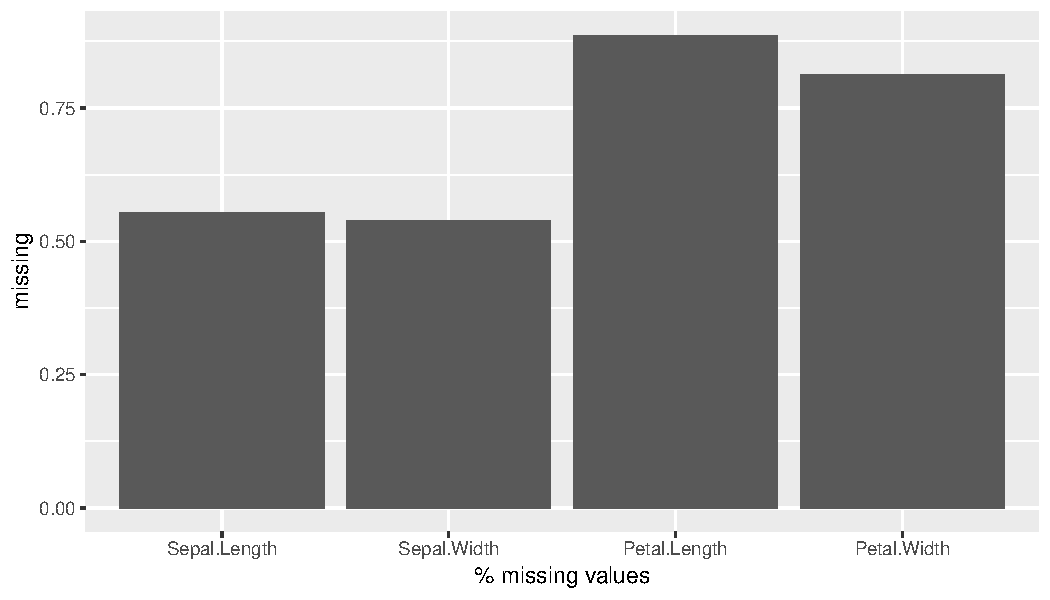
\includegraphics[width=0.8\textwidth]{plots/iris_data_missingness.pdf}
	\caption{Marginal share of missing values per covariate using the MAR strategy described in Equation~\eqref{eq:missing_strategy} and $\beta = (0, 0.2, 0.4, -0.2, -0.2)$.}
	\label{fig:marginal_missing}
\end{figure}

\subsection{Performance Comparison}\label{performance_comparison}
The predictive performance of the EM algorithm is compared to the strategies proposed in Section~\ref{traditional_methods}. Additionally, a decision tree based on the fully observed data is included as a reference for the best possible performance given the dataset and general modeling strategy. 
The results of a 10 fold cross validation are plotted in Figure~\ref{fig:performance}. The accuracy was computed on predictions of fully observed variables.
The EM algorithm performs similarly to the full data set and clearly outperforms the model only using observations without any missing values or imputing marginal means.
%
\begin{figure}[hp]
	\centering
	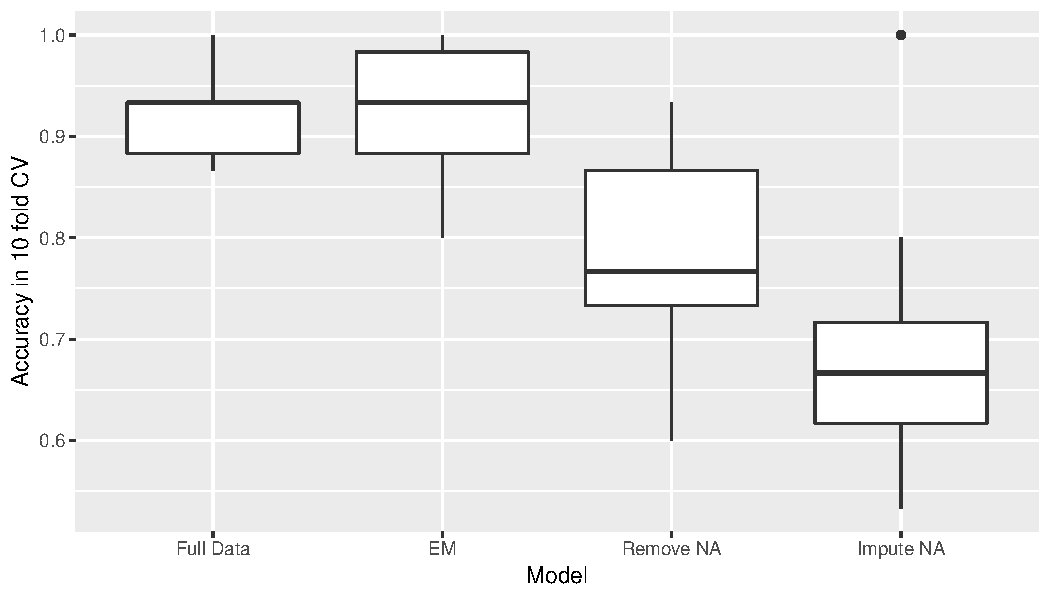
\includegraphics[width=0.8\textwidth]{plots/performance.pdf}
	\caption{Boxplots of the performance per fold of the classification tree based on the original data without missing values (Full Data), imputation using the EM algorithm proposed in Section~\ref{treatment_of_missing_values_in_cart} (EM), using only observations without missing values (Remove NA), and imputing marginal means (Impute NA).}
	\label{fig:performance}
\end{figure}
%
The average performance across the 10 folds of the cross validation is summarized in Table~\ref{tab:performance}. This shows that the proposed EM algorithm is capable of recovering high-dimensional dependencies in a data set with missing values, which results in an improved predictive power in comparison to simpler methods ignoring the MAR structure in the missing values.
\begin{table}[ht]
\caption{Average accuracy across the 10 fold cross validation 
of the classification tree, see Figure~\ref{fig:performance}.}
\centering
\begin{tabular}{r|llll}
 & Full Data & EM & Remove NA & Impute NA \\ 
\hline 
Accuracy & 0.93 &  0.93 &  0.79 &  0.69
\end{tabular}
\label{tab:performance}
\end{table}


% iris data figure
\begin{landscape}
 \begin{figure}
  \centering
  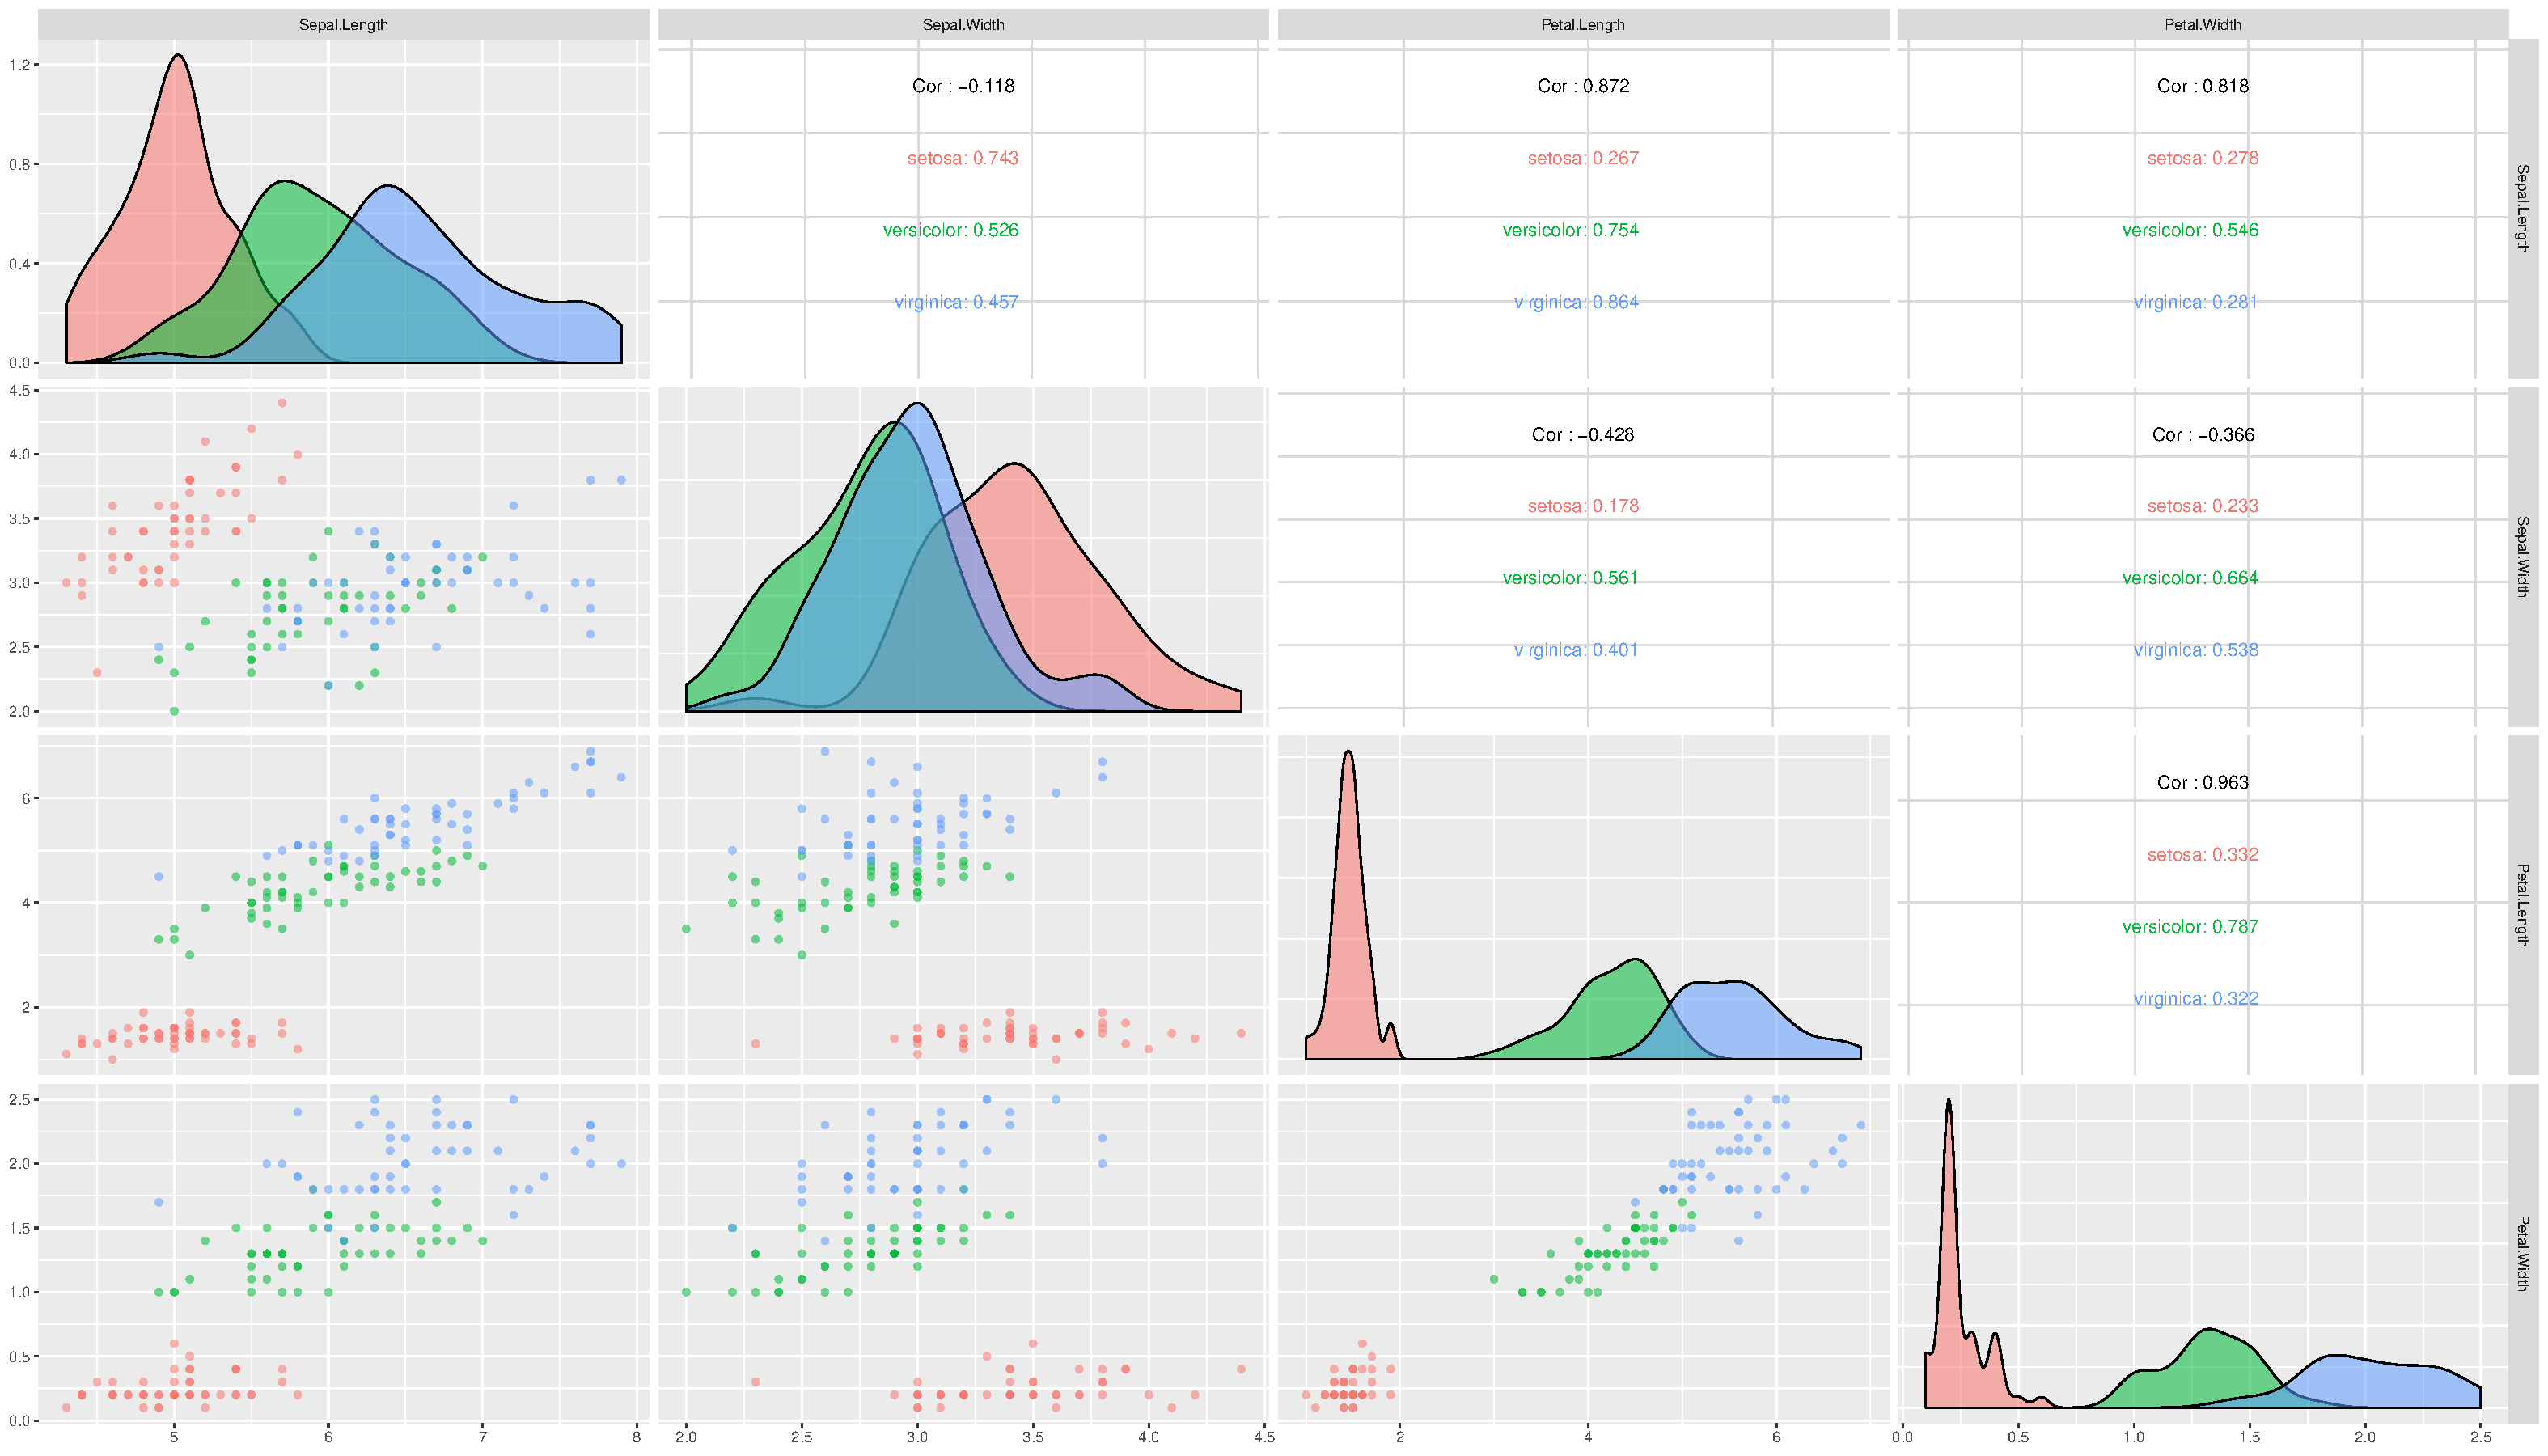
\includegraphics[height=0.8\textwidth]{plots/iris_data.pdf}
  \caption{Iris data: Density of the covariates per species on the diagonal, scatterplots between all covariates in the sub-diagonal plots, and overall and within species correlation coefficients of the covariates in the upper-diagonal plots.}
  \label{fig:iris}
 \end{figure}
\end{landscape}


\section{Future Research}\label{futre_research}

A high-yield expansion of this project is to generalize the proposed EM algorithm to Random Forests. Random forests are an ensemble of decorrelated CARTs \citep{breiman} that generally has increased predictive power in comparison with CART.
The EM algorithm for the entire ensemble would simplify to applying the EM algorithm proposed in Section~\ref{EM_for_CART} separately to each of the CARTs in the ensemble. This should result in similar performance improvements.

Generalizing the proposed EM algorithm to data with missing values in the target variable is straight forward. In the E step of the algorithm proposed in Section~\ref{treatment_of_missing_values_in_cart}, missing values in the target variable would be assigned to the mean/mode of the observations in the leaf node they fall into. This should work reasonably well for observations missing their target variable for which relevant covariates are fully observed. This would place the originally mislabeled observation into a leaf node with a majority of its actual class, which would lead to a reclassification in the E step. A similar strategy could also be used to predict labels for observations with missing values in covariates.

A variation on the proposed algorithm would be to create a Gibbs sampler that samples missing values from the marginal distribution  of the observed values in the corresponding leaf node. This would lead to slower convergence, but should reduce the probability of getting stuck in a local maximum of the distribution due to the random initial assignment.






%%%%%%%%%%%%%%%%%%%%%%%%%%%%%%%%%%%%%%%%%%%%%%%%%%%%%%%%%%%%%%%%%%%%%

\clearpage
\bibliographystyle{dcu} 
{\bibliography{bibliography.bib}}

%%%%%%%%%%%%%%%%%%%%%%%%%%%%%%%%%%%%%%%%%%%%%%%%%%%%%%%%%%%%%%%%%%%%%

\clearpage
\begin{appendix}
\appendix
\section*{Digital Appendix}
The R code implementing the EM algorithm proposed in Section~\ref{treatment_of_missing_values_in_cart} and the simulation study described in Section~\ref{simulation_study} can be found in the publicly accessible Github repository \url{https://github.com/maierhofert/EMforCART.git}. 
It also contains all figures and the Latex code used to generate this report.

\end{appendix}
\end{document}











\iffalse

\subsection{Data Generating Process}
The methodology proposed in Section~\label{treatment_of_missing_values_in_cart} is compared using a simulations study.
As the data generating process, an underlying two-dimensional random variable $(\tilde X, \tilde Y, C)$ is drawn as
\begin{eqnarray}
\tilde X \iid U[0, 1], \nonumber \\
\tilde Y \iid U[0, 1],
\end{eqnarray}
with class labels 
\begin{eqnarray}
C = 
\begin{cases}
1 & \text{ for } -0.5 < X < 0.5, \\
2 & \text{ for } X \leq -0.5 \text{ or } X \geq 0.5,
\end{cases}
\end{eqnarray}
see Figure~\ref{fig:simu_data} (top).
%
The observed random variables $(X, Y, C)$ are observations of $(\tilde X, \tilde Y, C)$ with added random noise, 
\begin{eqnarray}
X = \tilde X + \varepsilon_x, \nonumber \\
Y = \tilde Y + \varepsilon_y, \nonumber \\
\varepsilon_x, \varepsilon_y \iid N(0, 1),
\end{eqnarray}
see Figure~\ref{fig:simu_data} (middle).


\subsection{Introduction of Missing Values}
For the purpose of this simulation missing values were introduced at random (MAR). The probability of missing observation $X_i$ or $Y_i$ is sampled to be proportional to $X_i$ or $Y_i$, i.e.\
$$P(X_i \text{ missing}) \propto X_i.$$
Whether or not an observations contains missing values is depicted in the bottom of Figure~\ref{fig:simu_data}. Note that more 
%
\begin{figure}[hp]
	\centering
	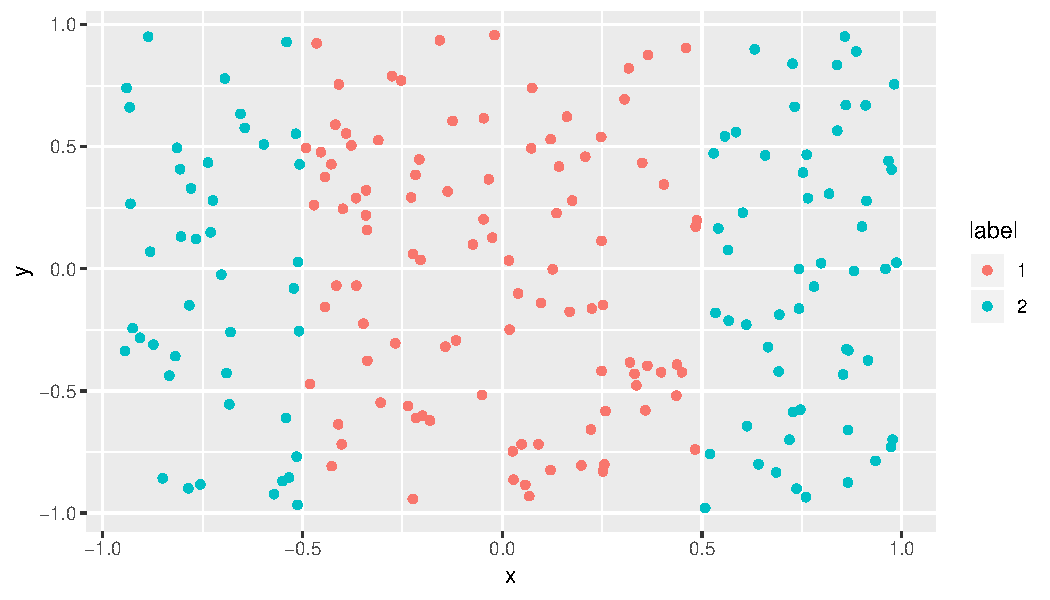
\includegraphics[width=0.8\textwidth]{plots/dat_underlying.pdf}
    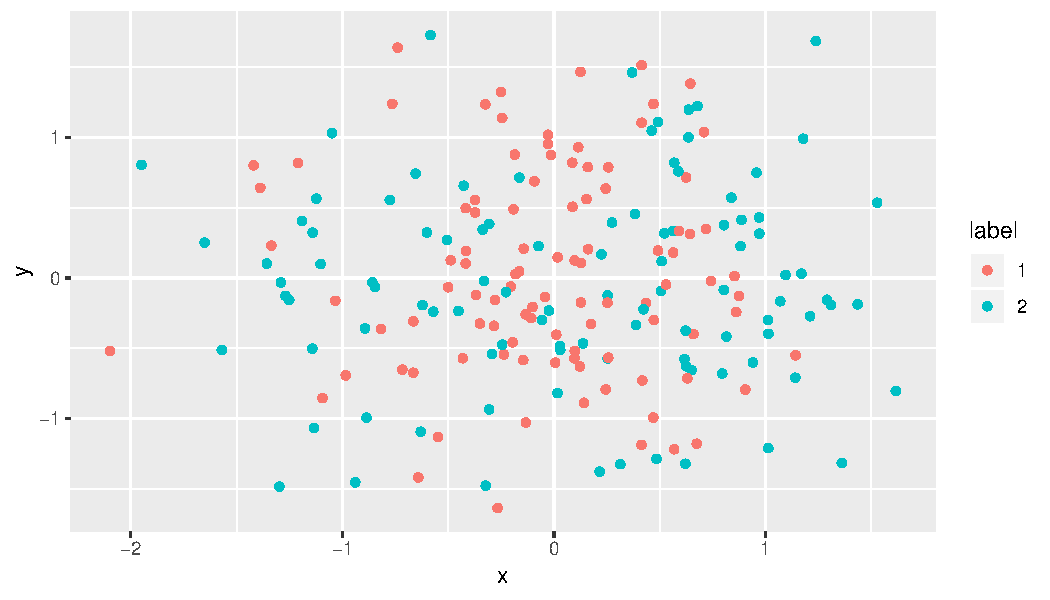
\includegraphics[width=0.8\textwidth]{plots/dat.pdf}
    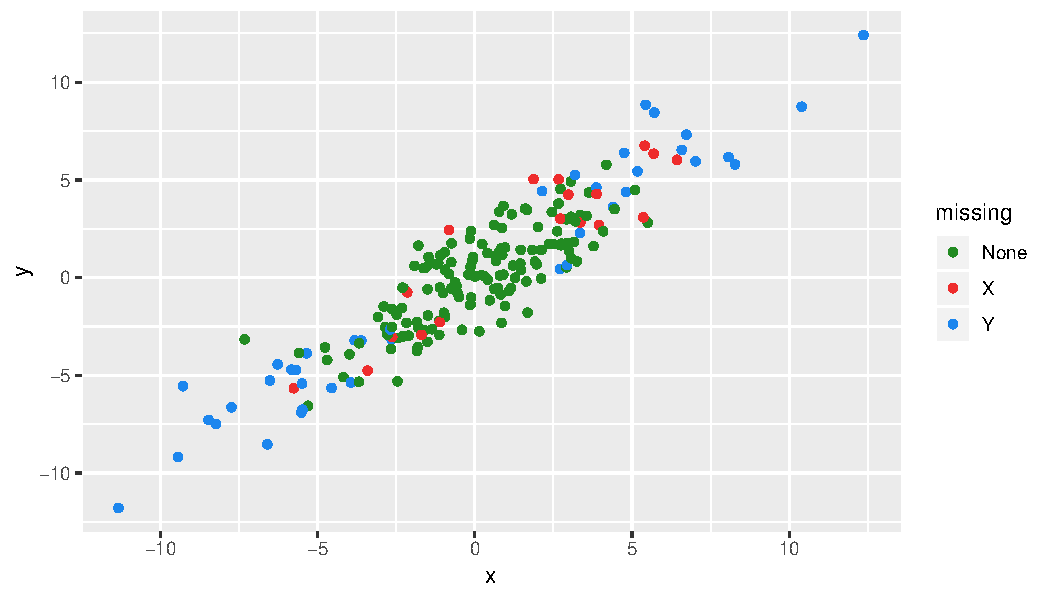
\includegraphics[width=0.8\textwidth]{plots/dat_MAR.pdf}
	\caption{Simulated data: Underlying data generating process (top) and noisy data (middle). Bottom: Observations with at least one missing value are colored in red, fully observed data in green.}
	\label{fig:simu_data}
\end{figure}


\fi